% !TEX root = C:/university/year_FS22/et2_labor/sw4/report/main.tex
\documentclass[11pt,a4paper]{article}
\usepackage{preamble}

% [VISUAL STUDIO CODE]-------------------
% I recommend setting an output path for the 'Latex Workshop' extension.
% I use following path, which generates the output into a 'output' folder:
% 
% {
%  "latex-workshop.latex.outDir": "%WORKSPACE_FOLDER%\\output"
% }
% 
% ---------------------------------------

% CONFIGURATION
% here you can change basic infos about the document.
\author{Joel von Rotz}
\date{19.03.2022}
\title{Aufbau eines Magnetfeldes}

% =============================================================================
\begin{document}

% TITLE PAGE/BLOCK 
$if(title)$
\title{$title$$if(thanks)$\thanks{$thanks$}$endif$}
\def\myTitle{$title$}
$endif$
$if(subtitle)$
\def\subtitle{$subtitle$}
$endif$
\author{$for(authors)$$it.name.literal$$sep$ \and $endfor$}
\date{$date$}
$if(beamer)$
$if(institute)$
\institute{$for(institute)$$institute$$sep$ \and $endfor$}
$endif$
$if(titlegraphic)$
\titlegraphic{\includegraphics{$titlegraphic$}}
$endif$
$if(logo)$
\logo{\includegraphics{$logo$}}
$endif$
$endif$



\begin{quote}
  \textsf{\textbf{Fragestellung:} Wie kann ein Magnetfeld mit einer Stärke von $H = \SI{0.25}{\milli\tesla}$ innerhalb eines Raums von mindestens $V = \SI{500}{\centi\metre^{3}}$ mit einer Spule erzeugt werden?}
\end{quote}

% \subsection{Gegebene Werte}

% \begin{equation}
%   l = \SI{0.25}{\metre} ; 
%   {\mu}_0 = 4 \cdot \pi \cdot 10^{-7} ; 
%   r = \SI{0.05}{\metre} ; 
%   B_0 = \SI{0.25}{\milli\tesla} ; 
%   I_{MAX} = \SI{0.9}{\ampere} ; 
%   d_{CU} = \SI{0.7}{\milli\metre}
% \end{equation}

% \begin{equation}
%   X_{L} = \omega \cdot L
% \end{equation}

% \begin{equation}
%   B_{0} = {\mu}_0\cdot \frac{N \cdot I}{l} \Rightarrow N = \frac{B_0\cdot l}{I \cdot {\mu}_0}
% \end{equation}

% \begin{equation}
%   N = \frac{0.25 \cdot 0.25}{0.9 \cdot 4 \cdot \pi \cdot 10^{-7}}= 55.26 \approx 56\ Windungen
% \end{equation}

% \begin{equation}
%   R_{CU} = \frac{\rho \cdot l}{A}
% \end{equation}


% SECTIONS
\subfile{sections/01_introduction.tex}
\subfile{sections/02_expectation.tex}
\subfile{sections/03_measuring_circuit.tex}
\subfile{sections/04_results.tex}
%\subfile{sections/05_deviations.tex}
\subfile{sections/06_conclusion.tex}
\section{Eigenständigkeitserklärung}

Hiermit versichere ich, dass die vorliegende Arbeit selbständig und ohne andere als die angegebenen Quellen und Hilfsmittel verfasst habe.

\begin{figure}[h]
  \centering
  \input{assets/sign_ine.pdf_tex}
  \label{sign_line} 
\end{figure}
\newpage
\section{Anhang}
\subsection{Bilder}
\begin{figure}[h]
  \centering
  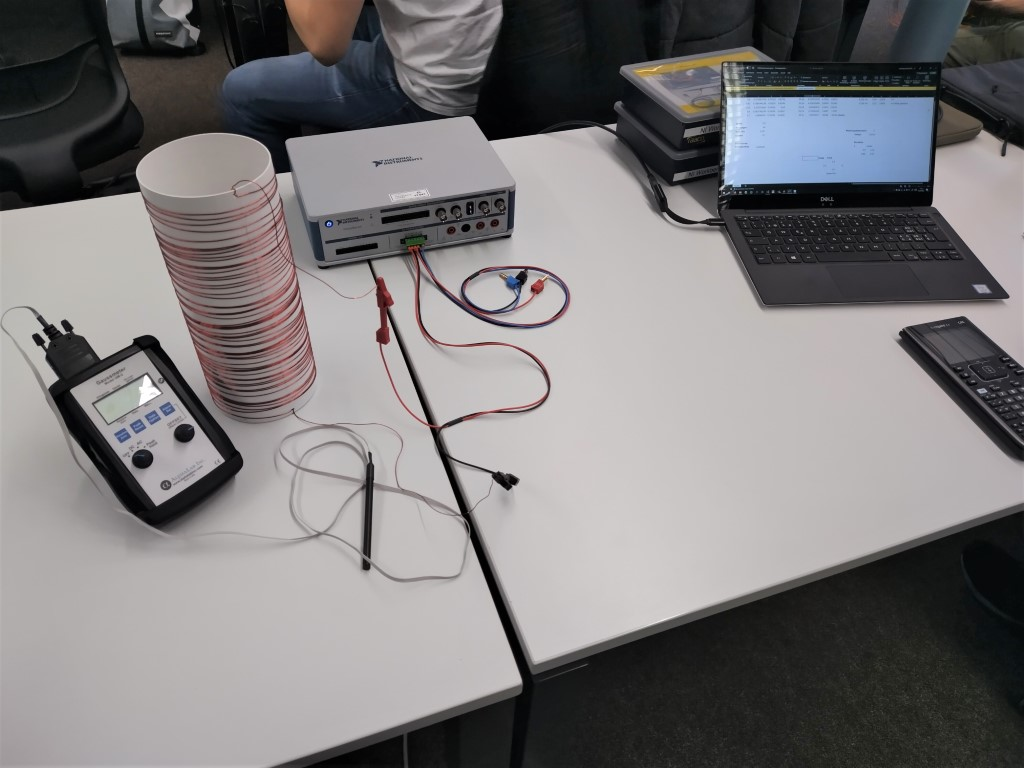
\includegraphics[scale=0.55]{assets/IMG_20220318_113714.jpg}
  \caption{Messungsaufbau (Das Bild zeigt vertauschte Speisungs-Kabel und die Spule ist auf dem Kopf $\Rightarrow$ Das Foto wurde erst am Schluss gemacht, nachdem noch anderes ausprobiert wurde mit der Spule)}
  \label{<label>}
\end{figure}
\end{document}
